\documentclass{beamer}
\mode<presentation>
%%Import
%\usepackage[ngerman]{babel}
\usepackage[utf8]{inputenc}
\usepackage{graphicx}
\usepackage{listings}
\usepackage{hyperref}

%%Layout
\usetheme{Singapore}
\usecolortheme[cmyk={1,0.7,0,0}]{structure}
%\setbeamercovered{transparent}
\beamertemplatenavigationsymbolsempty
\setbeamertemplate{footline}[frame number]

%%Meta-Daten
\title{Midterm Presentation - Safety Car}
\subtitle{HW/SW-Co-design with (LEGO)Cars}
\author{Florian, Feng, Chris and Lukas}
\institute[TUM]{Technische Universität München}
\date{2nd December 2013}
\logo{
\includegraphics[scale=0.5]{LogoFMI.png}}

\begin{document}

\begin{frame}
	\titlepage
\end{frame}

\begin{frame}
	\frametitle{Content}
	\tableofcontents
\end{frame}

\section{HW Setup}

\subsection{Car-Design}

\begin{frame}
	\frametitle{Hardware Overview}
	Key-Components:
	\begin{itemize}
		\item \textit{wooden chassis}, aprox. 40 cm x 35 cm
		
		\item \textit{12.6 V battery} with continuous 90 A ($\Rightarrow$ 1134 W!)\\
		Central power-management\\
		(generating 5 V for FPGAs and 9 V for Ethernet-Switch)	
	
		\item \textit{4 CMWUnits} (ControlMotorWheel-Unit) see next slide...
		
		\item \textit{Central FPGA} which controls every CMWUnit and sensor
		
		\item different \textit{Sensors}
	\end{itemize}
\end{frame}

\begin{frame}
	\frametitle{Car Design - Overview}
	\begin{figure}
	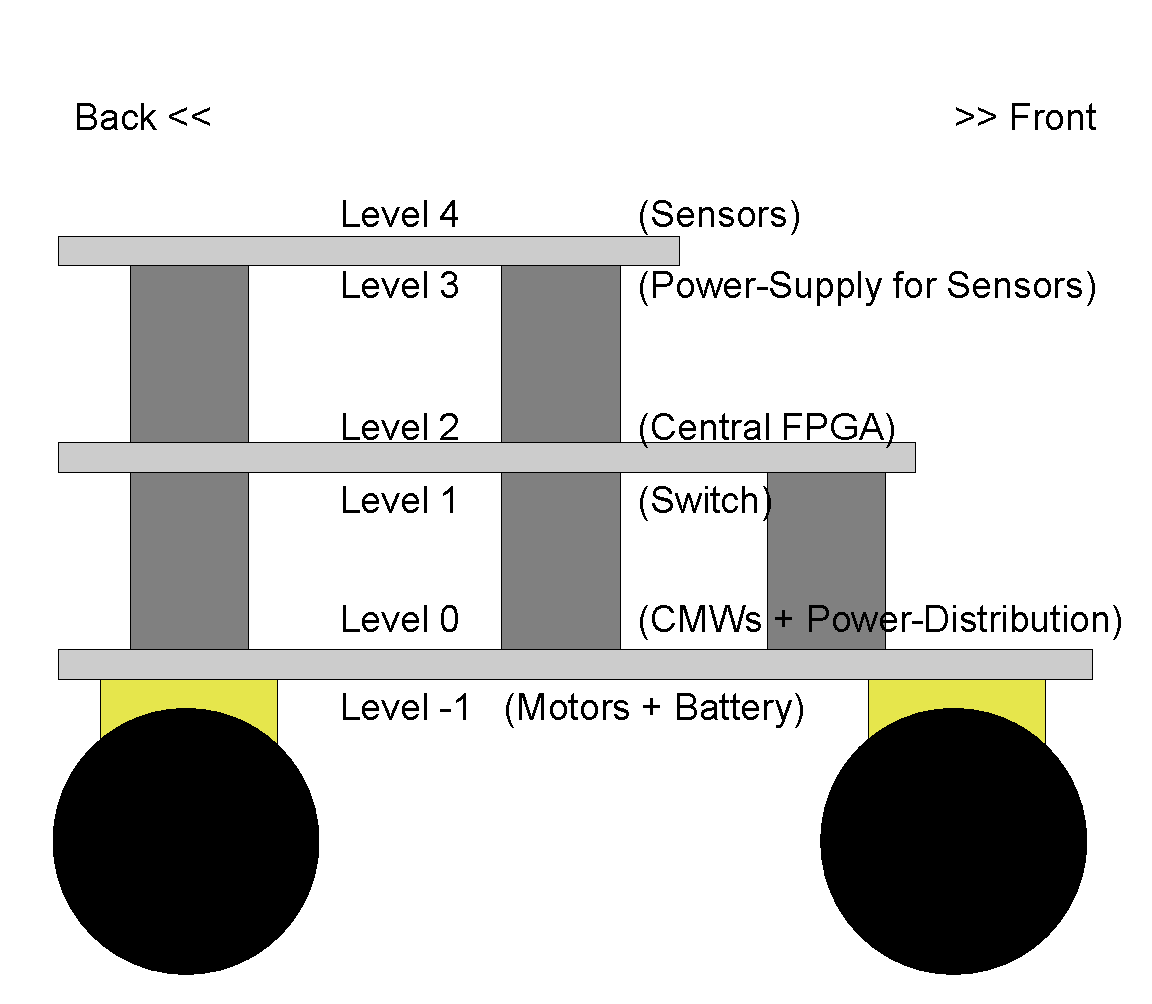
\includegraphics[scale=0.4]{figures/overview.pdf}
	\caption{The car is divided into five levels. Each level has a different motto.}
	\end{figure}
\end{frame}

\begin{frame}
	\frametitle{Level -1}
	The lowest level contains the four motors and the battery.
\end{frame}

\begin{frame}
	\frametitle{Level 0}
	\begin{figure}
	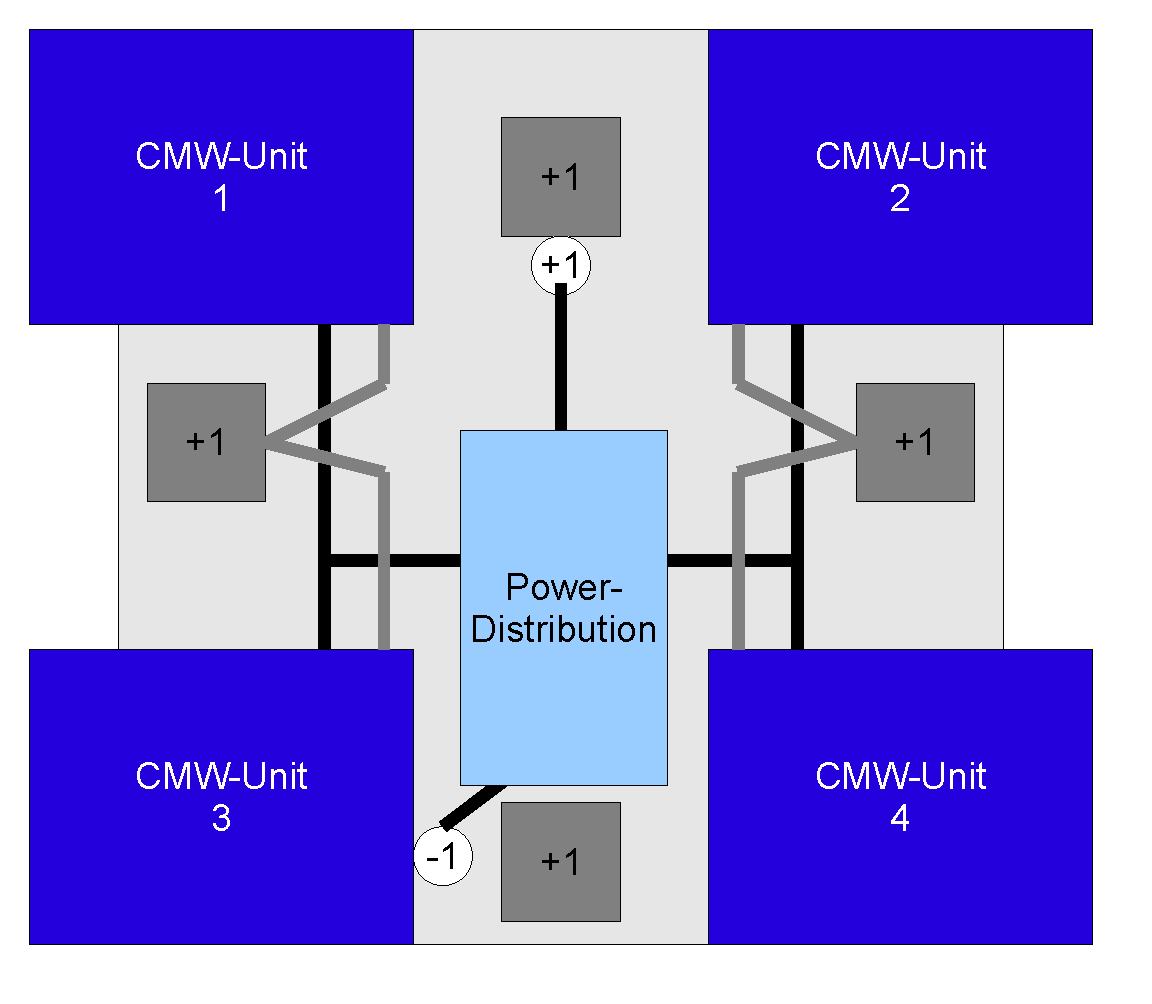
\includegraphics[scale=0.4]{figures/level0.pdf}
	\caption{Level 0 contains the CMW-Units and the Voltage-Distribution}
	\end{figure}
\end{frame}

\begin{frame}
	\frametitle{CMWUnit - Control-Motor-Wheel-Unit}
	Each Control-Motor-Wheel(CMW)-Unit consists of:
	\begin{itemize}	
		\item One \textit{Ethernet-UART} connected to the central FPGA
	
		\item One \textit{DE0Nano-Boards} (FPGA)
		
		\item One \textit{H-Bridge}	(dual-channel but we only use one channel)
	
		\item One \textit{Pololu Motor} (max. power: 60 W @ 12 V, 5 A).\\
		Problem: Many components can not take over 2 A! 
		
		\item One \textit{Soft-Wheel} (diameter: aprox. 12 cm)\\
		Problem: Each Soft-Wheel can take max. 3 kg 
	\end{itemize}
\end{frame}

\begin{frame}
	\frametitle{CMWUnit - Control-Motor-Wheel-Unit}
	\begin{figure}
	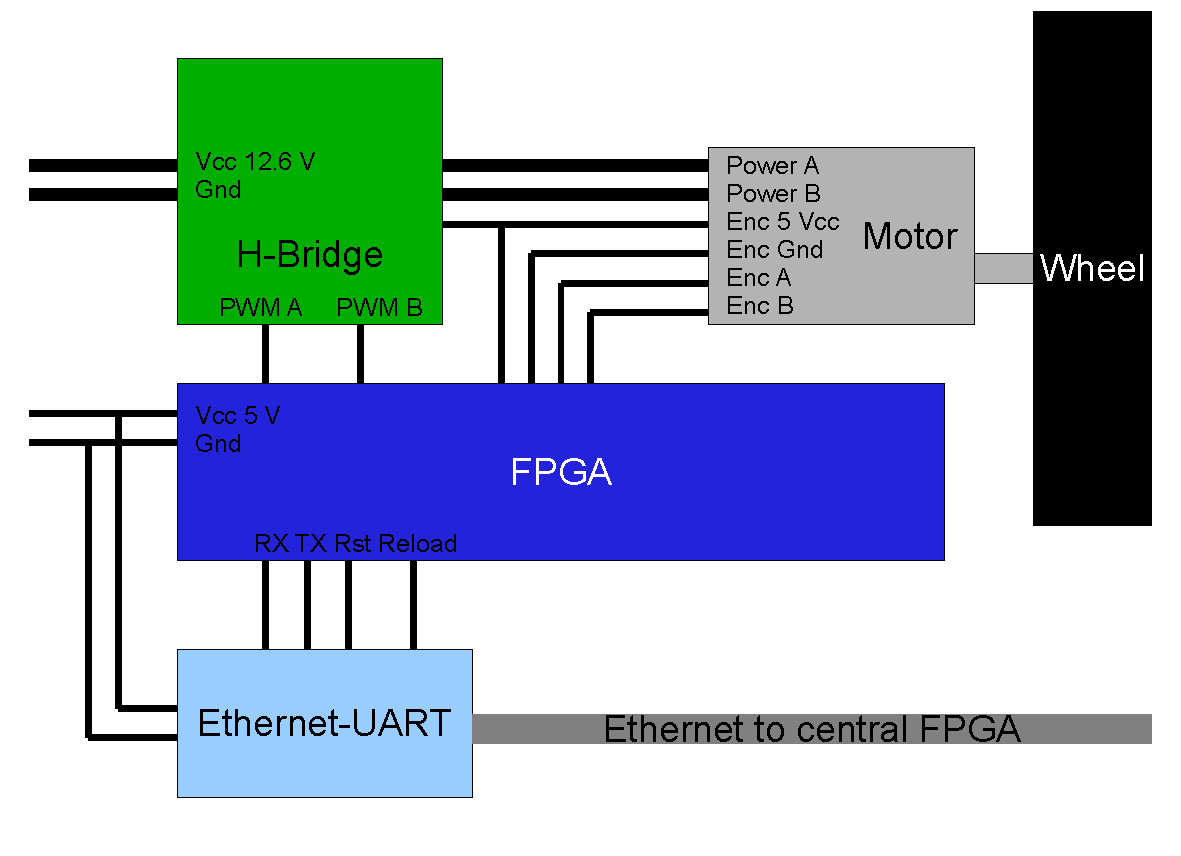
\includegraphics[scale=0.5]{figures/cmwunit.pdf}
	\caption{Interconnections in the Control-Motor-Wheel-Unit}
	\end{figure}
\end{frame}

\begin{frame}
	\frametitle{Level 1}
	\begin{figure}
	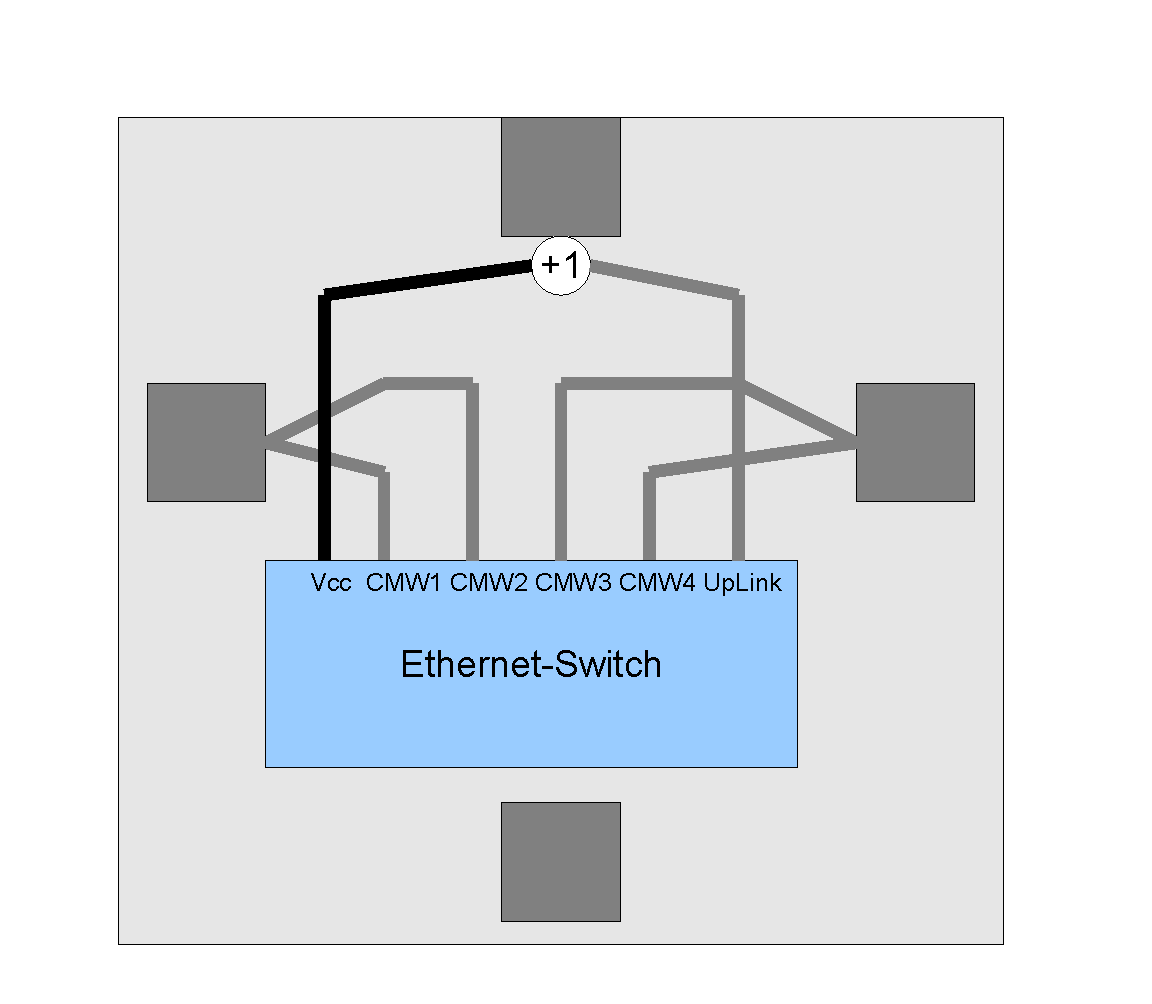
\includegraphics[scale=0.4]{figures/level1.pdf}
	\caption{Level 1 contains the Ethernet-Switch}
	\end{figure}
\end{frame}

\begin{frame}
	\frametitle{Level 2}
	\begin{figure}
	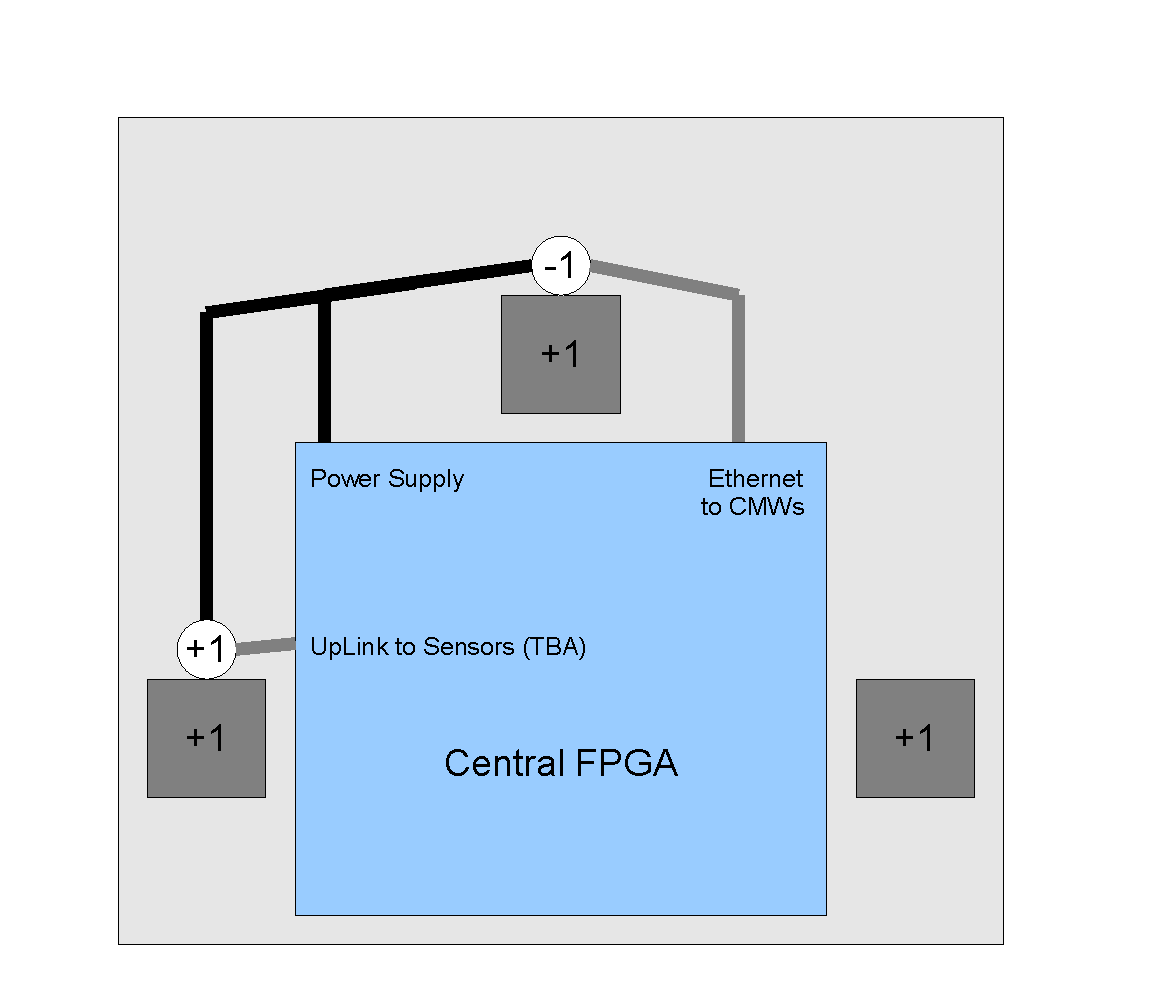
\includegraphics[scale=0.4]{figures/level2.pdf}
	\caption{Level 2 contains the (big) Central-FPGA}
	\end{figure}
\end{frame}

\begin{frame}
	\frametitle{Level 3}
	\begin{figure}
	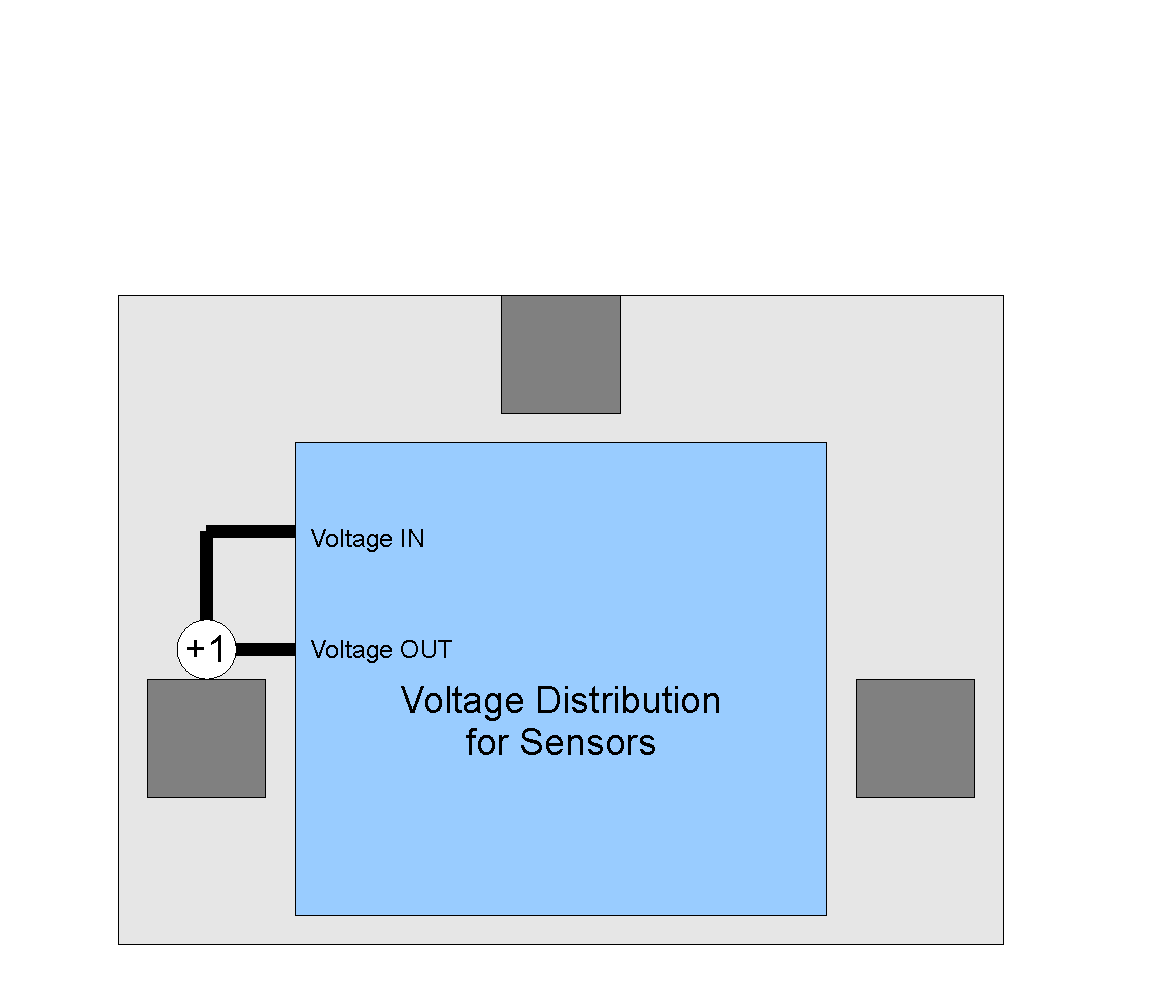
\includegraphics[scale=0.4]{figures/level3.pdf}
	\caption{Level 3 contains the Power-Supply for the Sensors}
	\end{figure}
\end{frame}

\begin{frame}
	\frametitle{Level 4}
	\begin{figure}
	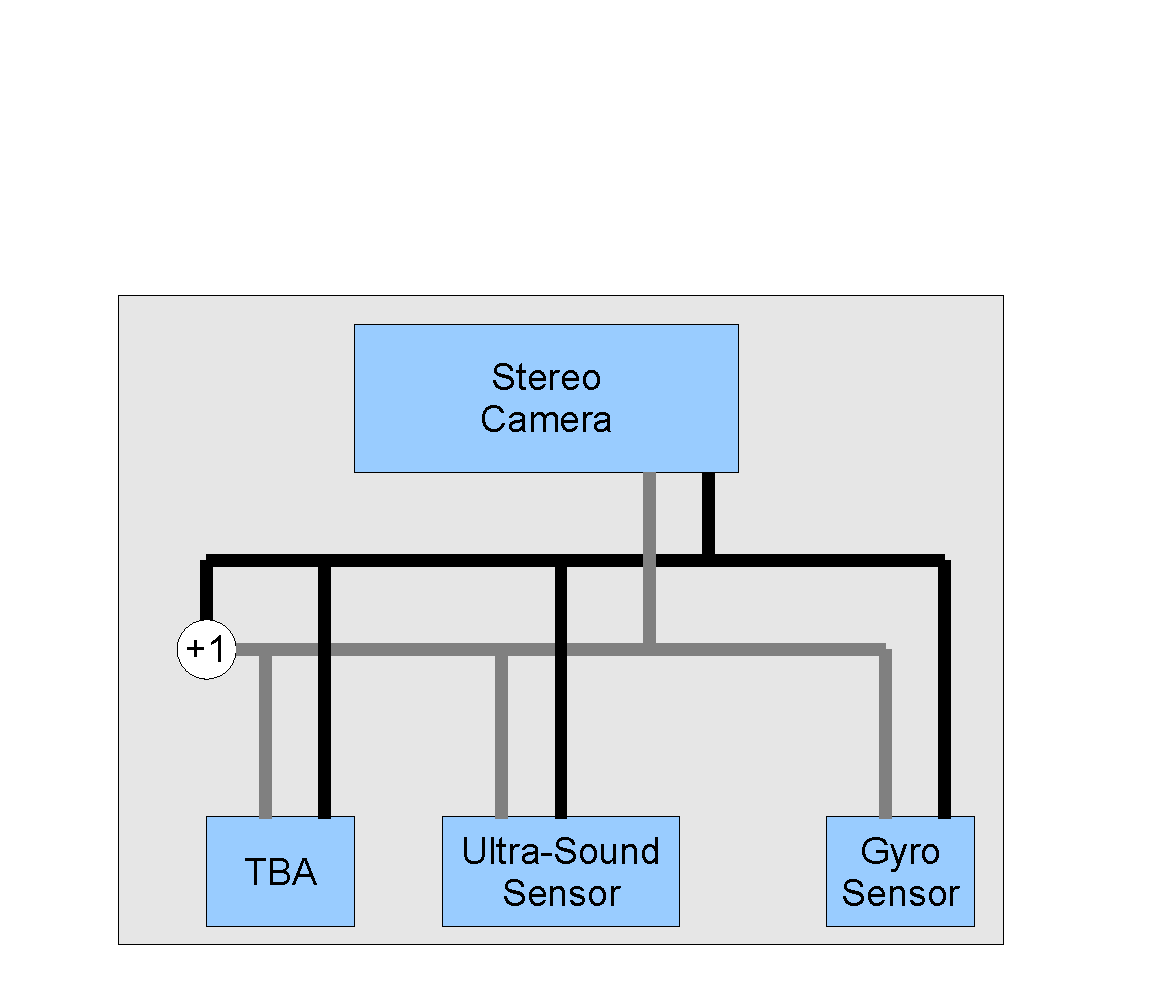
\includegraphics[scale=0.4]{figures/level4.pdf}
	\caption{Level 4 contains the Sensors}
	\end{figure}
\end{frame}

\subsection{Sensors}

%.........

\section{SW Architecture}

\subsection{Our Aims}
\begin{frame}
	\frametitle{Our Aims}
	We want to reach these architectural aims:
	\begin{enumerate}
		\item hierarchical and distributed System\\
		(e.g. separated Motor-Control)
		\item Plug-N-Play functionality \\
		(interactive protocols, drivers, ...)
		\item self-maintaining car \\
		(calibration mode, no hardcoded constants, ...)
		\item simple programming of the master-controller (FPGA)\\
		(e.g. Drag-N-Drop, ...)
	\end{enumerate}
\end{frame}

%\section{Networking}
%\subsection{Network Architecture}
%
%\begin{frame}
%	\frametitle{Network Architecture}
%	\begin{itemize}
%		\item single star-architecture
%		\item components communicate only with the central FPGA, not each other
%		\item components only understand the protocols they need
%		\item[] exception: CarIP (main protocol) and CarPNP (Plug-N-Play protocol)
%		\item similar components can use different protocols\\
%		(e.g. CMW-Units from different producers)
%	\end{itemize}
%\end{frame}
%
%
%\subsection{Communication-Protocols}
%\begin{frame}
%	\frametitle{CarIP - Car-Intranet-Protocol}
%	\begin{figure}
%	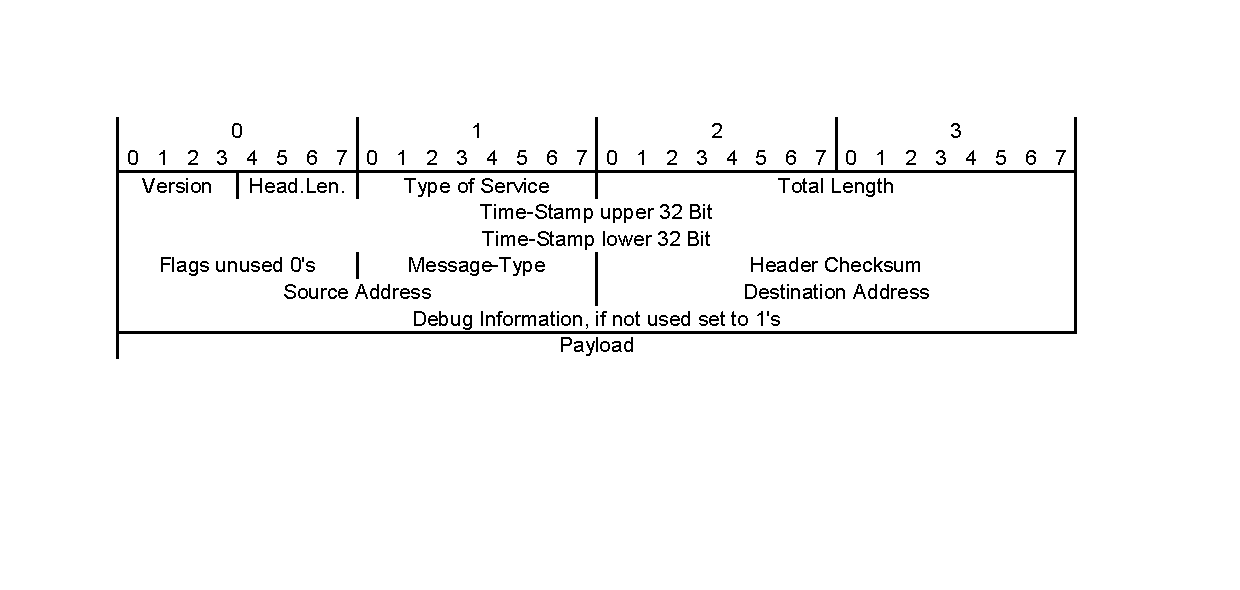
\includegraphics[scale=0.6]{figures/CarIP.pdf}
%	\caption{CarIP is the main transport protocol and behaves like IPv4}
%	\end{figure}
%\end{frame}
%
%\begin{frame}
%	\frametitle{CarIP - Car-Intranet-Protocol}
%	Features of CarIP:
%	\begin{itemize}
%		\item 64 Bit Time-Stamp (ns since 01.01.1970)
%		\item variable Message-Type and Payload (max. 65503 Bytes)
%		\item Address spitted in 8 Bit Component- and 8 Bit Sub-Component-Address.\\
%		Important if one FPGAs contains more controllers, ...
%		\item Debug- and/or Status-Information for networking
%	\end{itemize}
%\end{frame}
%
%
%\begin{frame}
%	\frametitle{CarPNP - Plug-N-Play-Protocol}
%	\begin{figure}
%	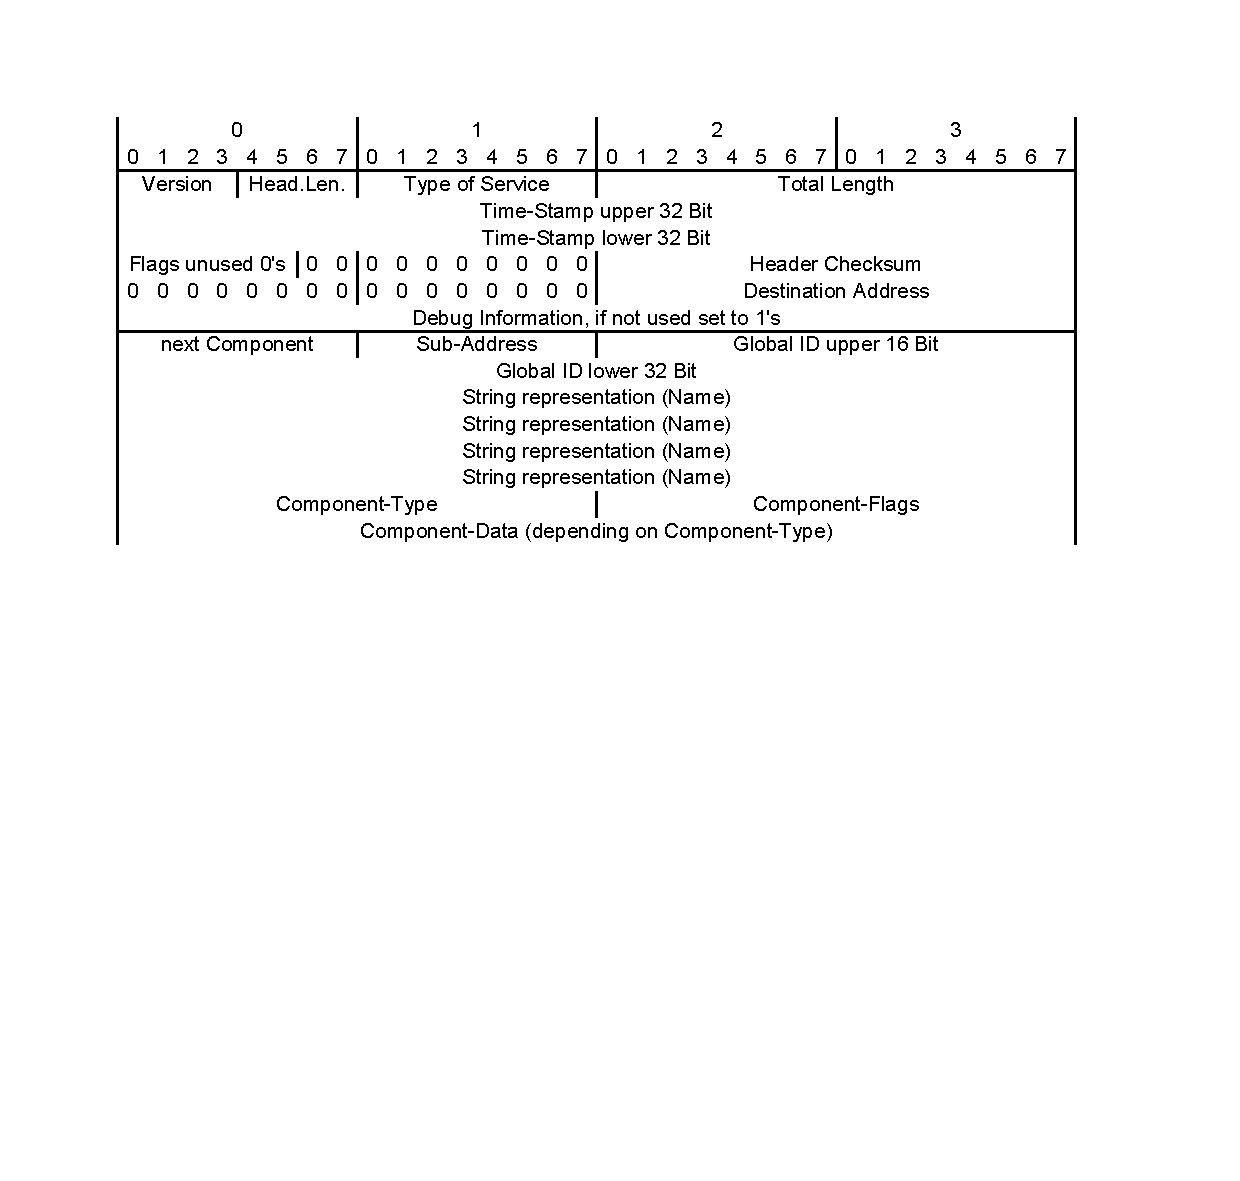
\includegraphics[scale=0.6]{figures/CarPNP_hello.pdf}
%	\caption{CarPNP-Hello - The sub-components are listed like a single-linked list }
%	\end{figure}
%\end{frame}
%
%\begin{frame}
%	\frametitle{CarPNP - Plug-N-Play-Protocol}
%	\begin{figure}
%	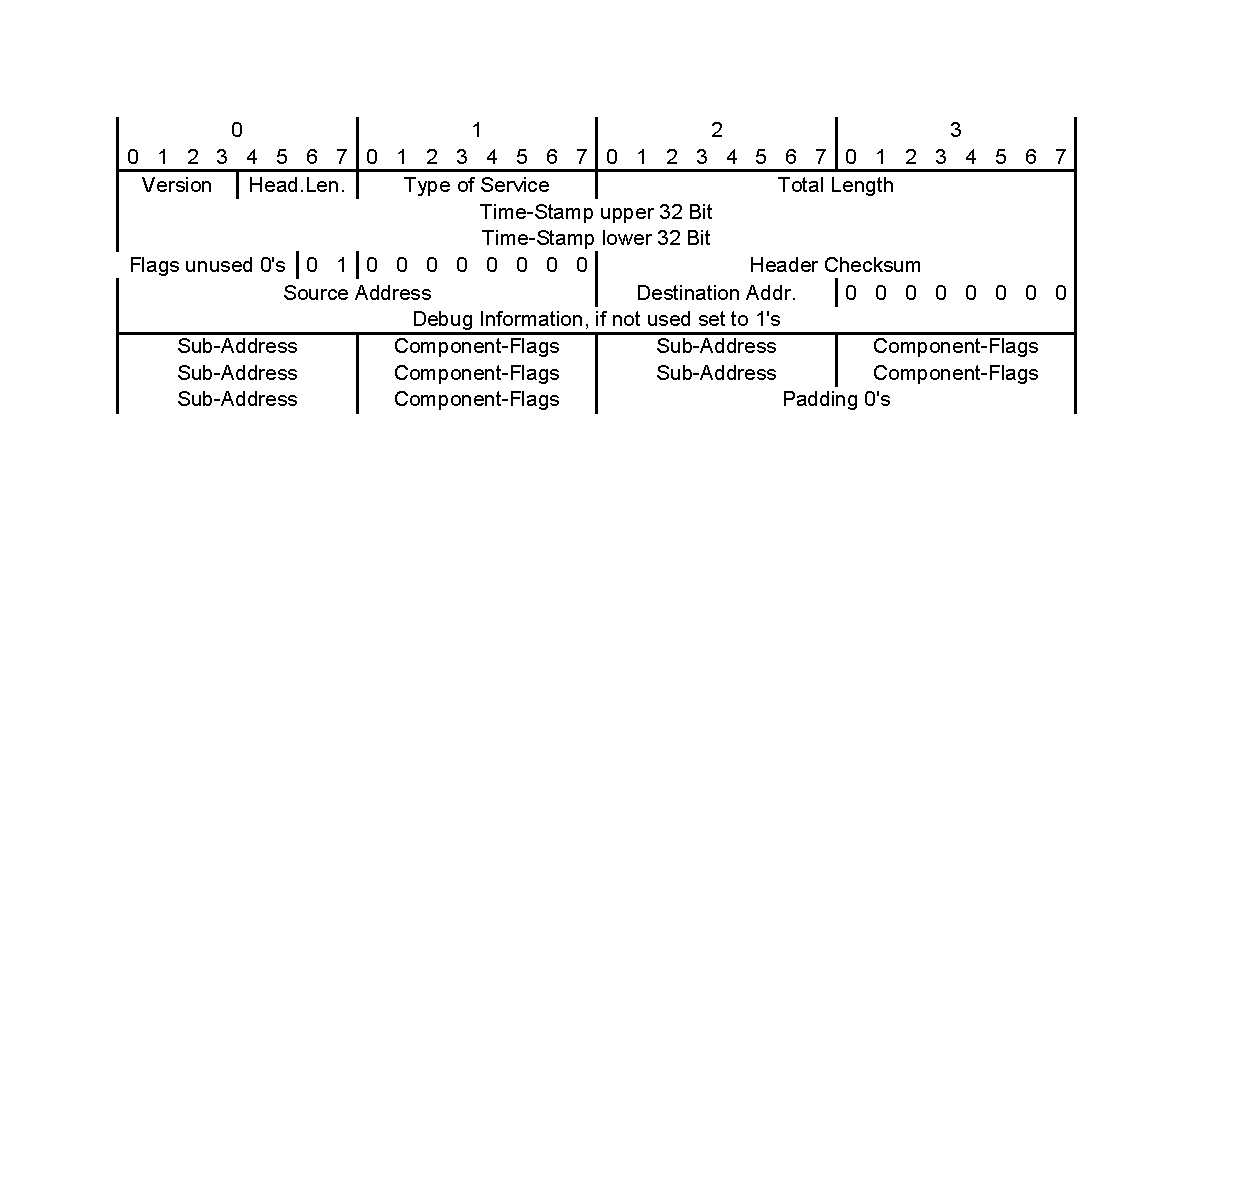
\includegraphics[scale=0.6]{figures/CarPNP_welcome.pdf}
%	\caption{CarPNP-Welcome - The sub-components get their sub-component-address }
%	\end{figure}
%\end{frame}
%
%\begin{frame}
%	\frametitle{CarPNP - Plug-N-Play-Protocol}
%	Features of CarPNP:
%	\begin{itemize}
%		\item variable count of sub-components
%		\item each sub-component can be described\\
%	 	(e.g. vMax, weight, sensor-distance, ...)
%		\item no hard-coded addressing
%	\end{itemize}
%\end{frame}

\section{Planned Features}

\end{document}
